\section{Метод Нелдера-Мида}

\textbf{Алгоритм метода}:
\begin{enumerate}

\item Задается начальная система точек (многогранник), включающий в себя $n + 1$ точку: $x^{0(1)}, x^{0(2)}, \ldots, x^{0(n+1)} $ (для функции 2-х переменных задается три начальные точки: $x^{0(1)}, x^{0(2)}, x^{0(3)} $).
\item Вычисляется значение функции во всех точках многогранника и выбирается:\\
лучшая точка $x^{(l)}: f(x^{(l)}) = \min_{i}|f(x^{k(i)})|$ (здесь $k$ --- номер итерации, $i$ --- номер точки)\\
худшая точка $x^{(x)}: f(x^{(x)}) = \max_{i}|f(x^{k(i)})|$

Далее заданная система точек перестраивается, для этого:

\item Строится центр тяжести системы заданных точек за исключением худшей:
$$ x^{(c)} = \dfrac{1}{n} \left( \sum_{i=1}^{n = 1} x^{k(i)} - x^{x} \right)$$
(для функции 2-х переменных точка $x^{(c)}$ --- середина отрезка, соединяющего точки за исключением худшей).

\item Выполняется операция отражения худшей точки через центр тяжести:
$$ x^{(o)} = x^{(c)} + \alpha (x^{(c)} - x^{(x)})$$
здесь $\alpha > 0$ --- параметр отражения (рекомендуемое значение $\alpha = 1$).

\item Формируется новая система точек (многогранник). Для этого в точке $x^{(o)}$ вычисляется значение функции, полученное значение сравнивается с $f(x^{(l)})$:

\begin{itemize}
\item если $f(x^{(o)}) < f(x^{(l)})$ выполняется операция растяжения:
$$ x^{(r)} = x^{(c)} + \gamma (x^{(o)} - x^{(c)})$$
здесь $\gamma > 0 (\gamma \neq 0)$ --- параметр растяжения (рекомендуемое значение $\gamma \in [2, 3]$).

При этом если $f(x^{(r)}) < f(x^{(o)})$, то в новой системе точек точка $x^{(x)}$ будет заменена на $x^{(r)}$, если же $f(x^{(r)}) \geq f(x^{(o)})$, то в новой системе точек точка $x^{(x)}$ будет заменена на $x^{(o)}$.

\item если $f(x^{(l)} \geq f(x^{(o)})  < f(x^{(x)})$ выполняется операция сжатия:
$$x^{(s)} = x^{(c)}) + \beta (x^{(x)}) - x^{(c)}))$$
здесь $\beta > 0 (\beta \neq 0)$ --- параметр сжатия (рекомендуемое значение $\beta \in [0.4, 0.6]$).

При этом если $f(x^{(s)}) < f(x^{(o)})$, то в новой системе точек точка $x^{(x)}$ будет заменена на $x^{(s)}$, если же $f(x^{(s)}) \geq f(x^{(o)})$, то в новой системе точек точка $x^{(x)}$ будет заменена на $x^{(o)}$.

\item если $f(x^{(o)}) \geq f(x^{(x)})$ выполняется операция редукции: при этом формулируется новый многогранник, содержащий точку $x^{(l)}$ с уменьшенными вдвое сторонами:
$$ x^{k+1(i)} = x^{(l)} + 0.5 (x^{k(i)} - x^{(l)}), i = 1, \ldots, n + 1$$.
\end{itemize}

Т.о. в результате выполнения этого пункта алгоритма формируется новая система точек (многогранник), причем в случае возникновения операций растяжения и сжатия перестраивается только одна точка --- $x^{(x)}$, в случае возникновения операции редукции --- все точки, за исключением $x^{(l)}$.

\item Процедуры $2 - 5$ повторяются до выполнения критерия окончания счета.
\end{enumerate}

Основной критерий окончания метода: $\sqrt{\dfrac{1}{n + 1} \sum_{i = 1}^{n + 1} |f(x^{k(i)}) - f(x^{(c)})|^{2}} \leq \varepsilon$

Начальные параметры метода: $x^{0(1)}, x^{0(2)}, \ldots, x^{0(n+1)}, \varepsilon $.

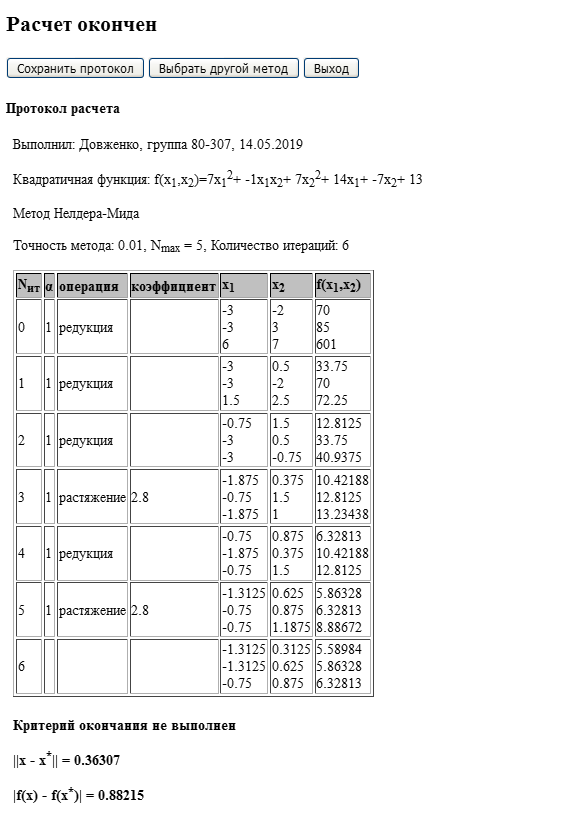
\includegraphics[width=0.8\linewidth]{om_hw_01/img/4.PNG}\\
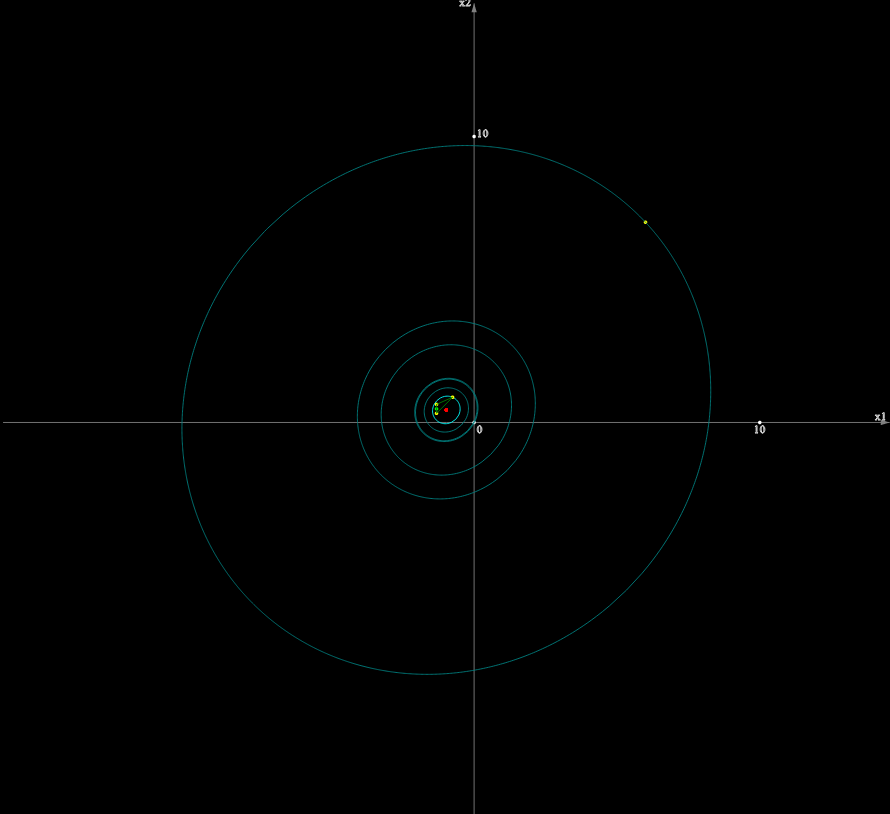
\includegraphics[width=\linewidth]{om_hw_01/img/4_2.PNG}\\

\pagebreak